%\documentclass{beamer} %voce pode usar este modelo tambem
\documentclass[t,handout,9pt]{beamer}
\usepackage{graphicx}
\usepackage{url}
\usepackage[british]{babel}
%\batchmode
% \pgfpagesuselayout{4 on 1}[letterpaper,landscape,border shrink=5mm]
\usepackage{amsmath}
\usepackage{amssymb}
\usepackage{amsfonts}
\usepackage{enumerate}
\usepackage{epsfig}
\usepackage{bbm}
\usepackage{calc}
\usepackage{adjustbox}
\usepackage{color}
\usepackage{ifthen}
\usepackage{capt-of}
\usepackage{float}
\usepackage{booktabs}
\usepackage{dcolumn}
\usepackage{multicol}
\usepackage{hyperref}
\usepackage[flushleft]{threeparttable}
\usepackage{subcaption}
\usepackage{adjustbox}
\usepackage{ragged2e}
\usepackage{pgfpages}
%\usepackage{showframe}

\usepackage{cmbright}

\renewcommand\ttdefault{cmvtt} % selects CM typewriter

\usepackage[utf8]{inputenc} % Required for inputting international characters
\usepackage[T1]{fontenc} 	% Output font encoding for international characters

%\DeclareFontShape{OT1}{cmss}{b}{n}{<->ssub * cmss/bx/n}{}

\usetheme[compress]{Berlin}
\definecolor{sapienza}{RGB}{0, 49, 83}
\usecolortheme[named=sapienza]{structure}

\usepackage[backend=bibtex,style=alphabetic,giveninits=true,url=false,eprint=false,doi=false]{biblatex}
\DeclareNameAlias{sortname}{last-first}
\renewcommand*{\nameyeardelim}{\addcomma\addspace}
\renewcommand*{\bibfont}{\footnotesize}
\addbibresource{example.bib}
\setbeamerfont{footnote}{size=\tiny}

\setbeamerfont{title}{size=\LARGE}

% reduce spaces between tables/figures and caption
\usepackage[font=small,skip=1pt]{caption}

%% pgf plots stuff
%\usepackage{pgfplots}
%\pgfplotsset{compat=newest}
%% the following commands are needed for some matlab2tikz features
%\usetikzlibrary{plotmarks}
%\usetikzlibrary{arrows.meta}
%\usepgfplotslibrary{patchplots}

% one navigation dot per slide trick
\AtBeginSection[]{\subsection{}}

% fix misbehave for allowframebreaks
\usepackage{etoolbox}
\makeatletter
\patchcmd{\slideentry}{\ifnum#2>0}{\ifnum2>0}{}% replace the subsection number test with a test that always returns true
% use frame numbers instead of subsection slide numbers so that frames broken over slides get separate circles
\patchcmd{\slideentry}{\c@subsectionslide}{\c@framenumber}{}{\@error{unable to patch}}
\patchcmd{\beamer@writeslidentry}{\c@subsectionslide}{\c@framenumber}{}{\@error{unable to patch}}

% date in footer trick
\makeatletter
  \setbeamertemplate{footline}{%
    \begin{beamercolorbox}[colsep=1.5pt]{upper separation line foot}
    \end{beamercolorbox}
    \begin{beamercolorbox}[ht=2.5ex,dp=1.125ex,%
      leftskip=.3cm,rightskip=.3cm plus1fil]{author in head/foot}%
      \leavevmode{\usebeamerfont{author in head/foot}\insertshortauthor}%
      \hfill%
      {\usebeamerfont{institute in head/foot}\usebeamercolor[fg]{institute in head/foot}\insertshortinstitute}%
    \end{beamercolorbox}%
    \begin{beamercolorbox}[ht=2.5ex,dp=1.125ex,%
      leftskip=.3cm,rightskip=.3cm plus1fil]{title in head/foot}%
      {\usebeamerfont{title in head/foot}\insertshorttitle\hfill\insertshortdate}%
    \end{beamercolorbox}%
    \begin{beamercolorbox}[colsep=1.5pt]{lower separation line foot}
    \end{beamercolorbox}
  }
\makeatletter

% remove dot for titlepage and Outline
\makeatletter
\let\old@beamer@writeslidentry\beamer@writeslidentry
\def\beamer@writeslidentry{%
  \expandafter\beamer@ifempty\expandafter{\beamer@framestartpage}{}% does not happen normally
  {%else
    \clearpage\beamer@notesactions%
  }
}
\makeatother

% let's number figure captions
\setbeamertemplate{caption}[numbered]

% trick for grouping equations
\newenvironment{rcases}
  {\left.\begin{aligned}}
  {\end{aligned}\right\rbrace}

%-------------------------Titulo/Autores/Orientador------------------------------------------------
\title[Introduction to Computer Programming]{Introduction to Computer Programming}
\date[A.Y. 2024-2025]{\\A.Y. 2024-2025}
\author[Alessio Martino]{Prof. Alessio Martino\\
\smallskip
{\small \href{mailto:amartino@luiss.it}{\texttt{amartino@luiss.it}}}\\
\smallskip
}
\institute[10/09/2024]{Department of Business and Management\\Viale Romania 32, 00197 Rome\\[\bigskipamount]

\includegraphics[scale=0.4]{Figures/cliente-luiss.png}%
}

%-------------------------Logo na parte de baixo do slide------------------------------------------
%\pgfdeclareimage[height=0.7cm]{senac-logo}{senac-logo.pdf}
%\logo{\pgfuseimage{senac-logo}\hspace*{0.5cm}}

%-------------------------Este código faz o menuzinho bacana na parte superior do slide------------
%\AtBeginSection[]
%{
%  \begin{frame}<beamer>
%    \frametitle{Outline}
%    \tableofcontents[currentsection]
%  \end{frame}
%}
%\beamerdefaultoverlayspecification{<+->}
% -----------------------------------------------------------------------------

\begin{document}
% -----------------------------------------------------------------------------

%---Gerador de Sumário---------------------------------------------------------

\frame[noframenumbering]{
	\titlepage
}

% begin personalization stuff
\setbeamertemplate{navigation symbols}{%
	\insertslidenavigationsymbol
	\insertframenavigationsymbol
	\insertsubsectionnavigationsymbol
	\insertsectionnavigationsymbol
	\insertdocnavigationsymbol
	\insertbackfindforwardnavigationsymbol
	\hspace{1em}%
	\usebeamerfont{footline}
	\insertframenumber/\inserttotalframenumber%
}
\setbeamertemplate{itemize items}[circle]
\setbeamertemplate{enumerate items}[circle]
\setbeamertemplate{bibliography item}{\insertbiblabel}
% end personalization stuff

\section[]{}
\begin{frame}{Outline}
	\tableofcontents
\end{frame}
%\begin{frame}{Outline}
%\begin{multicols}{2}
%  \tableofcontents
%\end{multicols}
%\end{frame}
%---Fim do Sumário------------------------------------------------------------

% reset navigation dots for other slides
\makeatletter
\let\beamer@writeslidentry\old@beamer@writeslidentry
\makeatother

% -----------------------------------------------------------------------------
\section{What is Computation?}
\subsection{What does a Computer do?}
\begin{frame}{What is Computation?}
Well, basically:
\begin{itemize}
	\item \textcolor{red}{performs} calculations\\
	$\rightarrow$ a billion calculations per second!
	\item \textcolor{red}{remembers} results\\
	$\rightarrow$ hundreds of GigaBytes of storage!
\end{itemize}
\vfill
What kind of \textcolor{red}{calculations}?
\begin{itemize}
	\item built-in (`primitive') included in the programming language
	\item custom and ad-hoc defined by the programmer
\end{itemize}
\vfill
Humans are lazy!\\
Computers only do (and know) what you tell them.\\
\end{frame}
%
\subsection{Knowledge}
\begin{frame}
\vfill
Two major computing paradigms:
\begin{itemize}
	\item Declarative programming\\
	$\rightarrow$ statements of fact\\
	\qquad we describe \textit{what} task the program must accomplish
	\item Imperative programming\\
	$\rightarrow$ just like a recipe\\
	\qquad we describe \textit{how} the program must accomplish the task
\end{itemize}
\vfill
In many cases, code will be a mixture of both designs too, so it's not always black-and-white.
\vfill
\textcolor{red}{Imperative programming} is what we will see in this course.
\vfill
\end{frame}
%
\section{Recipe = Algorithm}
\begin{frame}{Recipe = Algorithm}
\vfill
An algorithm features:
\begin{itemize}
	\item a sequence of \textcolor{red}{simple steps}
	\item \textcolor{red}{flow of control} to specify when each step must be executed
	\item a way of determining when to \textcolor{red}{stop}.
\end{itemize}
\vfill
... just like a recipe!
\vfill
Even a plain $1+2+3+4+5=?$ is an algorithm!
\vfill
\end{frame}
%
\begin{frame}
A slightly more complex example: Newton's method.\\
The square root of $x$ is a number $y$ such that $y \cdot y = x$ $\leftarrow$ \textcolor{red}{declarative!}\\
Let's see an \textcolor{red}{imperative} version:
\begin{enumerate}
	\item start with a guess $g$
	\item if $g \cdot g$ is ``close enough'' to $x$\\
	\begin{enumerate}[a]
	\item let $y=g$
	\item stop
	\end{enumerate}
	\item otherwise\\
	\begin{enumerate}[a]
	\item let $g \leftarrow \frac{1}{2}\left( g + \frac{x}{g}\right)$
	\item repeat from step \#2
	\end{enumerate}
\end{enumerate}
\begin{table}[]
\centering
\caption{Square root of 16 via Newton's method}
\begin{tabular}{@{}ccc@{}}
\toprule
$g$    & $g \cdot g$                        & $\frac{1}{2}\left( g + \frac{x}{g}\right)$                      \\ \midrule
3      & $3 \cdot 3 =9$                     & $\frac{1}{2}\left( 3 + \frac{16}{3}\right) \simeq 4.17$         \\
4.17   & $4.17 \cdot 4.17\simeq 17.39$      & $\frac{1}{2}\left( 4.17 + \frac{16}{4.17}\right) \simeq 4.0035$ \\
4.0035 & $4.0035 \cdot 4.0035\simeq 16.028$ & $\frac{1}{2}\left( 4.0035 + \frac{16}{4.0035}\right) \simeq 4$  \\ \bottomrule
\end{tabular}
\end{table}
\end{frame}
%
\section{Inside a Computer}
\begin{frame}{Inside a Computer}
\vfill
Types of computing machines.\\
\begin{description}
	\item[Fixed-Program Computers:] machines designed to do very specific things.\\
	Notable examples:
	\begin{itemize}
		\item Alan Turing's bombe machine (1939--1940)
		\item Atanasoff-Berry computer (1942)
		\item Arithmetic calculators
	\end{itemize}
	\item[Stored-Program Computers:] machines able to store and manipulate sequences of instructions. \\
	Notable examples:
	\begin{itemize}
		\item Manchester Mk1 (1948--1949)
		\item any modern PC
	\end{itemize}
\end{description}
\vfill
\end{frame}
%
\begin{frame}
\vfill
\begin{figure}
	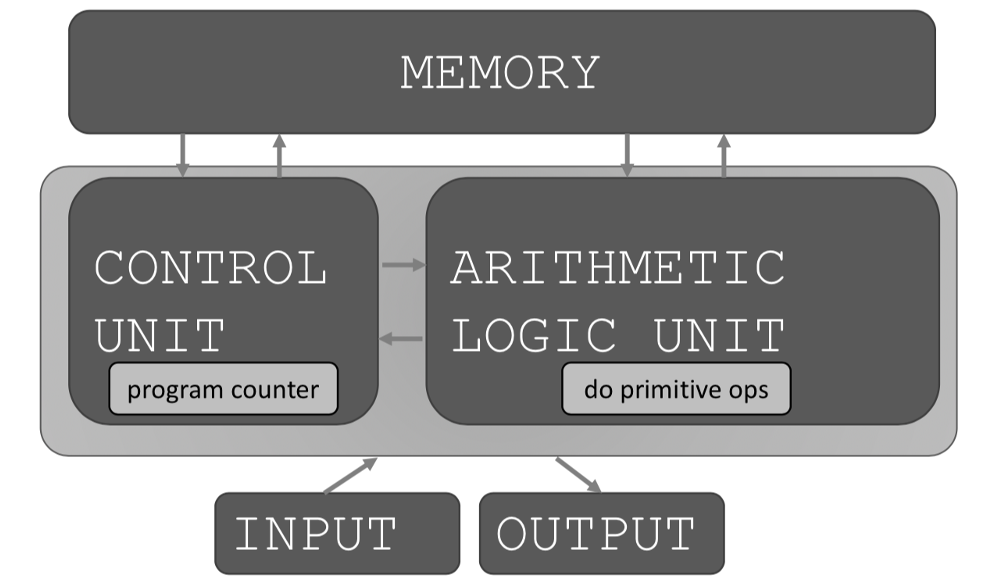
\includegraphics[width=\textwidth]{Figures/VNarch}
	\caption{Von Neumann architecture (circa 1945)}
\end{figure}
\vfill
\end{frame}
%
\begin{frame}
\vfill
Execution of instructions:
\begin{itemize}
	\item sequence of \textcolor{red}{instructions stored} inside the computer\\
	Build from primitive instruction-set:
	\begin{enumerate}
		\item arithmetic and logic
		\item simple tests
		\item moving data
	\end{enumerate}
	\item a special program (the \textit{interpreter}) \textcolor{red}{executes each instruction in order}:
	\begin{itemize}
		\item use simple tests to change the flow of the sequence, if needed
		\item stops when done.
	\end{itemize}
\end{itemize}
\vfill
\end{frame}
%
\begin{frame}
\adjustbox{valign=t}{\begin{minipage}{0.5\textwidth}
\vspace{1cm}
\begin{itemize}
\item Alan Turing in 1936 showed that you can \textcolor{red}{compute anything} using 6 primitives and a `Turing Machine': read/write/delete, move left/right, nowt.
\item Current programming languages have much higher-level set of primitives!
\item A programming language is said to be \textit{Turing complete} if it can be used to simulate a Turing Machine.
\item Current programming languages are Turing complete.
\end{itemize}
\end{minipage}}%
\hfill
\adjustbox{valign=t}{\begin{minipage}[t]{0.4\textwidth}
\vspace{0.5cm}
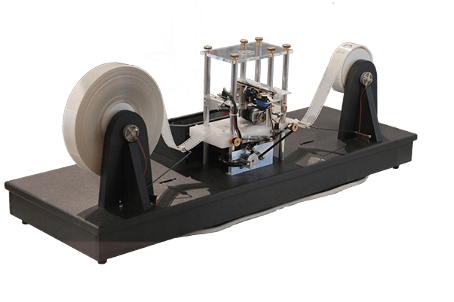
\includegraphics[width=\textwidth]{Figures/Turing1}
\newline\vspace{0.7cm}
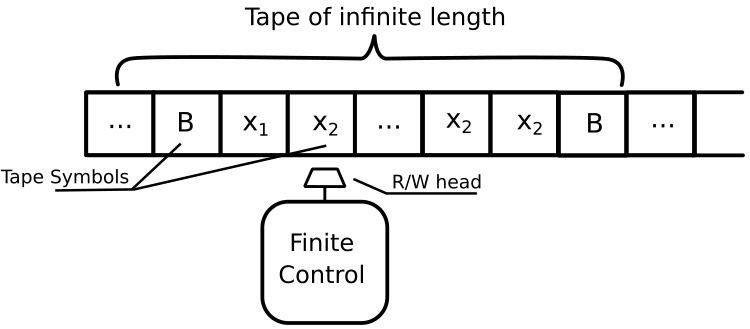
\includegraphics[width=\textwidth]{Figures/Turing2}
\end{minipage}}
\end{frame}
%
\section{Programming Languages}
\begin{frame}{Programming Languages}
\vfill
Luckily, we don't have Turing machines, tapes and headers.\\
\vfill
Common \textcolor{red}{programming languages} are much more comfortable, intuitive and easier to work with.\\
\vfill
A programming language:
\begin{itemize}
	\item provides a set of \textcolor{red}{primitive} operations;
	\item allows \textcolor{red}{expressions}, which are `valid' (and possibly complex) combinations of primitives;
	\item uses \textcolor{red}{values} in expressions and computations, which have \textcolor{red}{meanings}.
\end{itemize}
\vfill
\end{frame}
%
\begin{frame}
\vfill
Programming languages can be divided in two big families:\\
\begin{description}
	\item[High-level programming languages,] which are user-oriented (e.g., Java, C++, Python)
	\item[Low-level programming languages,] which are machine-oriented (e.g., binary, assembly)
\end{description}
\begin{figure}
     \centering
     \begin{subfigure}[b]{0.3\textwidth}
         \centering
         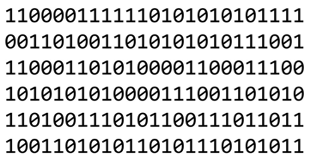
\includegraphics[width=\textwidth]{Figures/graph1}
         \caption{Binary}
     \end{subfigure}
     \hfill
     \begin{subfigure}[b]{0.3\textwidth}
         \centering
         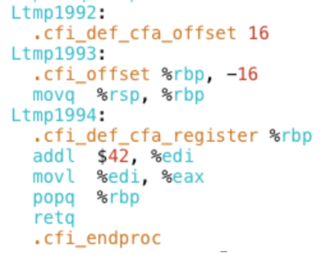
\includegraphics[width=\textwidth]{Figures/graph2}
         \caption{Assembly}
     \end{subfigure}
     \hfill
     \begin{subfigure}[b]{0.3\textwidth}
         \centering
         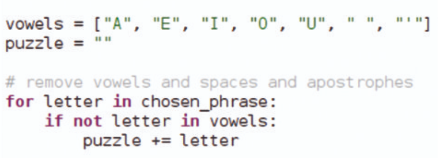
\includegraphics[width=\textwidth]{Figures/graph3}
         \caption{Python}
     \end{subfigure}
\caption{Example of high- and low-level programming languages}
\end{figure}
\vfill
\end{frame}
%
\subsection{Language Translation}
\begin{frame}
\begin{block}{Problem}
Computers understand binary code. How do we transform a program written in a high-level language into binary?
\end{block}
\adjustbox{valign=t}{\begin{minipage}{0.5\textwidth}
\vspace{0.5cm}
\begin{description}
\item[Interpreted:] A program that reads a high-level language and executes it one line at the time
\item[Compiled:] Reads the entire source code and converts it into a machine program (binary executable).
\item[Hybrid:] Translation into an intermediate byte-code, which is later interpreted.
\end{description}
\end{minipage}}%
\hfill
\adjustbox{valign=t}{\begin{minipage}[t]{0.4\textwidth}
\vspace{0.5cm}
\begin{figure}
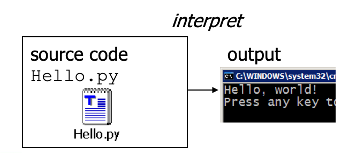
\includegraphics[width=\textwidth]{Figures/Interpreted1}
\caption{Interpreted}
\end{figure}
% \newline%\vspace{0.7cm}
\begin{figure}
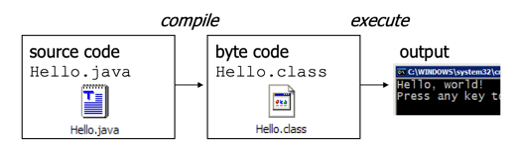
\includegraphics[width=\textwidth]{Figures/Interpreted2}
\caption{Hybrid/Compiled}
\end{figure}
\end{minipage}}%
\end{frame}
%
\subsection{Important Aspects of Programming Languages}
\begin{frame}
\vfill
\begin{itemize}
	\item Primitive Constructs
	\vfill
	\item Syntax
	\vfill
	\item Semantics
	\vfill
	\item Errors \& Bugs
\end{itemize}
\vfill
In order to explain these aspects, let's see some analogies with the English language.
\vfill
\end{frame}
%
\begin{frame}
\begin{center}\textcolor{red}{Primitive Constructs}\end{center}
\begin{description}
	\item[English:] words and punctuations
	\item[Programming Language:] simple operators, numbers, strings
\end{description}
\vfill
\begin{figure}
     \centering
     \begin{subfigure}[b]{0.3\textwidth}
         \centering
         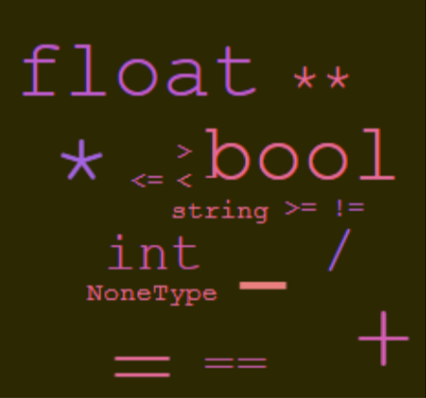
\includegraphics[width=\textwidth]{Figures/Primitive1}
         \caption{Python}
     \end{subfigure}
     \hfill
     \begin{subfigure}[b]{0.6\textwidth}
         \centering
         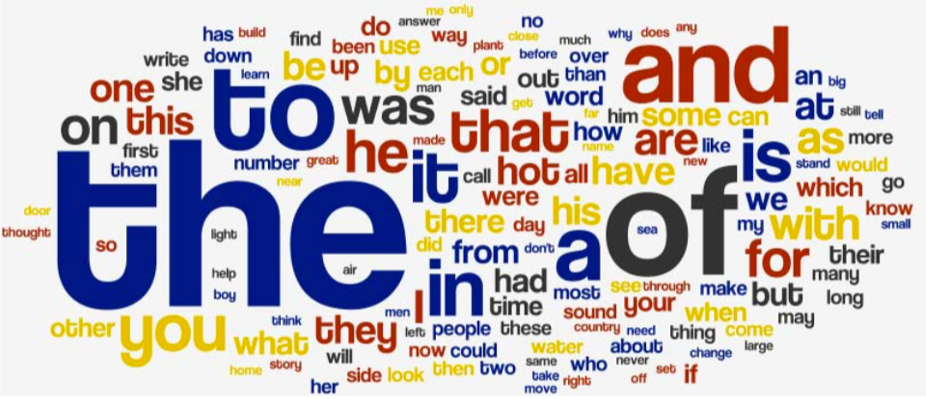
\includegraphics[width=\textwidth]{Figures/Primitive2}
         \caption{English}
     \end{subfigure}
\caption{}
\end{figure}
\end{frame}
%
\begin{frame}
\begin{center}\textcolor{red}{Syntax}\end{center}
The syntax of a language defines which strings of characters and symbols are well formed.
\begin{center}\textcolor{blue}{English}\end{center}
\texttt{``cat dog boy''} $\rightarrow$ not syntactically valid (<noun, noun, noun> is not allowed in English)\\
\texttt{``cat hugs boy''} $\rightarrow$ syntactically valid (<noun, verb, noun> is allowed in English)
\begin{center}\textcolor{blue}{Programming Language}\end{center}
\texttt{``hi''5} $\rightarrow$ not syntactically valid (concatenation of different data types)\\
\texttt{3.2 * 5} $\rightarrow$ syntactically valid (operands linked by operator)
\end{frame}
%
\begin{frame}
\begin{center}\textcolor{red}{(Static) Semantic}\end{center}
The static semantics defines which syntactically valid strings have a meaning.
\begin{center}\textcolor{blue}{English}\end{center}
\texttt{``I are big''} $\rightarrow$ syntactically valid (<pronoun, verb, adjective> is allowed in English)\\
\qquad\qquad \ \ $\rightarrow$ semantically wrong (\texttt{I} is singular, \texttt{are} is plural)
\begin{center}\textcolor{blue}{Programming Language}\end{center}
\texttt{3.2 / 'cat'} $\rightarrow$ syntactically valid (operands linked by operator)\\
\qquad\qquad \ \ $\rightarrow$ semantically wrong (cannot divide numbers by strings)
\end{frame}
%
\begin{frame}
\begin{center}\textcolor{red}{Semantic}\end{center}
The semantics of a language associates a meaning with each syntactically correct string of symbols that has no static semantic errors.
\begin{center}\textcolor{blue}{English}\end{center}
\texttt{``Flying planes can be dangerous''}\\
\begin{enumerate}
	\item It can be dangerous for a person to fly planes
	\item Planes flying in the air can be dangerous
\end{enumerate}
\begin{center}\textcolor{blue}{Programming Language}\end{center}
Expressions have only one meaning ... yet can differ from what the programmer expects!
\end{frame}
%
\begin{frame}
\vfill
\begin{description}
	\item[Syntax Errors:] common for beginners and easy to catch. Programming languages do not allow the program to start if Syntax Errors are caught.
	\item[(Static) Semantic Errors:] some programming languages check for such errors. Yet, if uncaught, can cause unexpected behaviour.
	\item[Semantic Errors:] If a program has no syntactic errors and no static semantic errors, it has semantics. However, that isn't to say that it has the semantics that its creator intended it to have. When a program means something other than what its creator thinks it means, bad things can happen (run forever, crash, uncertainty of the results).
\end{description}
\vfill
\end{frame}
%------------------------------------------------------------------------------
%\section{References}
%\begin{frame}[allowframebreaks]{References}
%%\bibliographystyle{apacite}
%\printbibliography[heading=none]
%\end{frame}
\section{References}
\begin{frame}{References}
\begin{itemize}
	\item Guttag, J. V. (2013). \textit{Introduction to Computation and Programming using Python (Revised and Expanded Edition)}. MIT Press. [Chapter 1, Intro to Chapter 2]
	\item Downey, A. (2015). \textit{Think Python}. Green Tea Press ed. 2nd. [Sections 1.1, 2.8 \& Appendix A]
\end{itemize}
\end{frame}
%------------------------------------------------------------------------------
\section{Acknowledgments}
\begin{frame}{Acknowledgments}
\begin{itemize}
	% \item Prof. Irene Finocchi (LUISS University)\\
	% \quad \textit{Introduction to Computer Programming} Lecture Notes (2020-2021)
	\item \url{https://iq.opengenus.org/general-introduction-to-turing-machine/}
\end{itemize}
\end{frame}
%------------------------------------------------------------------------------
%\subsection{Sites legais}
%\begin{frame}{Sites legais}
%  Want to know more? See!
%  \begin{itemize}
%    \item Browse in my page \url{http://www.ezefranca.com}.
%    \item Browse on BCC page \url{http://www.sp.senac.br/bcc}.
%    \item Thanks WriteLaTeX from Support! \url{http://www.writelatex.com}.
%  \end{itemize}
%
%\end{frame}
%------------------------------------------------------------------------------

% -----------------------------------------------------------------------------
\end{document}
%-----------------------------------------------Este comentario nunca aparecera
